\documentclass{article}

% If you're new to LaTeX, here's some short tutorials:
% https://www.overleaf.com/learn/latex/Learn_LaTeX_in_30_minutes
% https://en.wikibooks.org/wiki/LaTeX/Basics

% Formatting
\usepackage[utf8]{inputenc}
\usepackage[margin=1in]{geometry}
\usepackage[titletoc,title]{appendix}

% Math
% https://www.overleaf.com/learn/latex/Mathematical_expressions
% https://en.wikibooks.org/wiki/LaTeX/Mathematics
\usepackage{amsmath,amsfonts,amssymb,mathtools}

% Images
% https://www.overleaf.com/learn/latex/Inserting_Images
% https://en.wikibooks.org/wiki/LaTeX/Floats,_Figures_and_Captions
\usepackage{graphicx,float}

% Tables
% https://www.overleaf.com/learn/latex/Tables
% https://en.wikibooks.org/wiki/LaTeX/Tables

% Algorithms
% https://www.overleaf.com/learn/latex/algorithms
% https://en.wikibooks.org/wiki/LaTeX/Algorithms
\usepackage[ruled,vlined]{algorithm2e}
\usepackage{algorithmic}

% Code syntax highlighting
% https://www.overleaf.com/learn/latex/Code_Highlighting_with_minted
% \usepackage{minted}
%\usemintedstyle{borland}

% References
% https://www.overleaf.com/learn/latex/Bibliography_management_in_LaTeX
% https://en.wikibooks.org/wiki/LaTeX/Bibliography_Management
\usepackage{biblatex}
\addbibresource{references.bib}

\usepackage{hyperref}
\hypersetup{
    colorlinks=true,
    linkcolor=blue,
    filecolor=magenta,      
    urlcolor=cyan,
}

% Title content
\title{AMATH 582 Homework 1: Denoising Stationary Signal Using FFT}
\author{Hongda Li}
\date{\today}

\begin{document}

\maketitle

% Abstract
\begin{abstract}
    The paper seeks to explain the process of using FFT as a way to denoise static signal. Specially using the assumption of the presence of whitenosie within the data, we can leverage the statistic feature of normal distribution to reduce the amount of noise in the frquency domain. To demonstrate it, we were given the hypothetical scenario of searching for a submarine and synthetic data to work with, and the goal is to recover the full path of the submarine. 
\end{abstract}

% Introduction and Overview
\section{Introduction and Overview}
We are interested in locating a submaring in the Puget Sound area given some noisy acoustic data. The assignment is designed to test the skill of filtering out noise in stationary waves, with the reward of figuring out the full path that the submarine takes. 
\\
The data given is a cube of data, collection every 30 mins during a 24 hours period. The data is in the format of complex double and the magnitude of each of the data point represents the presence and absence of the submarine. And that is, if it's zoro then it marks its absence else it marks its presence. 

% % Example Subsection
% \subsection{Subsection Title}
% This is a subsection.

% % Example Subsubsection
% \subsubsection{Subsubsection Title}
% This is a subsubsection.

%  Theoretical Background
\section{Theoretical Background}
\subsection{Fourier Series/Transform, and Frequency Domain}
    As we learned from our textbook \cite{kutz_2013}, Fourier introduced the concept of representing a given function $f(x)$ by a trigonometric series of sines and cosines:
    \begin{equation}
        f(x) = \frac{a_0}{2} + \sum_{i=1}^\infty \left(a_n\cos{nx} + b_n\sin{nx}\right) \quad x \in (-\pi,\pi].
        \label{eqn:fourierseries}
    \end{equation}
    And the coefficients of the $\sin$ and $\cos$ is up to our interests because it transform the signal with additional useful mathematical properties. 
    The continuation of the Fourier Series is Fourier Transform: 
    \begin{equation}\label{eqn:fourier-transform}
        F(k) = \frac{1}{\sqrt{2\pi}}\int_{-\infty}^\infty
        \exp(-ikx)f(x) dx
    \end{equation}
    And the inverse Fourier Transform is: 
    \begin{equation}
        f(x) = \frac{1}{\sqrt{2\pi}}
        \int_{-\infty}^\infty \exp(ikx) F(k)dk
    \end{equation}
    The Fourier Transform extend the domain for the coefficients of $\sin$ and $\cos$ to the real domain. 
    \\
    For computational reasons, signal is discretized into $2^n$ floats and then a discrete Fourier Transform is performed on the signal. The algorithm is relatively efficient with $\mathcal{O}(N\log(N))$ complexity where $N$ is the length of the signal. 
    \\
    In addition, the Fourier Transform above is appicable for signal in $[-\pi, \pi]$ range, but in actual application, the signal locates in $[-L, L]$ or $[L/2, L/2]$ (depends on convention) range. The the additional caveats that, the FFT algorithm shifts the domain in its implementation. 
    \\
    Therefore, for any given signal in the domain $[-L/2, L/2]$, the multiplier $k$ equals to $\frac{2\pi}{L}$, and when the signal has been discretized: $k_i = \frac{2\pi i}{L}$ where $-\frac{N}{2}\le i< \frac{N}{2}$.
    \\
    Therfore, our frequency domain goes from $\frac{-\pi N}{L}$ to $\frac{\pi N}{L}$. 

\subsection{Denoising in the Frequency Domain}
    The idea here is to observe the same signal over different time frame of times and realize that the expected value of white nosie in the frequency domain is zero. This idea is Further Discussed in The data science textbook\cite{kutz_2013_pg316}.
    \\
    Let $\epsilon_i$ to be a white noise signal sampled with discretization of $N$, then: 
    \begin{equation}
        \Re(\widehat{\epsilon_i}) \sim\text{Normal}(0, \sigma) \wedge 
        \Im(\widehat{\epsilon_i}) \sim\text{Normal}(0, \sigma)
        \implies \mathbb{E}(\widehat{\epsilon_i}) = 0
    \end{equation}
    And this means that, summing over the same stationary signal over different time frame will reduce the magnitude of white noise in the frequencise domian because the real and imaginary part of the white noise has an expecation value of zero. 

\subsection{Filtering and Reconstruction of the Submarine Path}
    Because the signal is stationary, therefore the frequency component is unchanging, and in this particular case, the submarine emits a particlar frequency the is unknown. 
    \\
    Therefore after the denosing process, we seek to find the unknown frequencies by simply looking for the frequency compoenent that has maximum magnitude.
    \\
    After the identification of the signal, we use a Gaussian filter to boost this particular frequencies in the original signal. The Gaussian filter is given as: 
    \begin{equation}\label{eqn:gaussian-filter}
        \exp
        \left(\mu_x (x - x_i)^2 +
                \mu_y(y - y_0)^2
                +\mu_z(y - y_0)^2\right)
    \end{equation}
    Where $x_0, y_0, z_0$ is the frequencies we try to boost (Should be the singal that the submarine is emiting) and the multiplier $\mu_x, \mu_y, \mu_z$ determines the window size of the Gaussian filter. 
    \\
    After the desired signal emitted by the submarine is identified, using the gusssian filter and applied it to the signal in the fourier domain will allow us to listen to this particular frequency. A similar idea but for 1D signal is discussed in the textbook\cite{kutz_2013_pg312} , here we extend the same idea into 3D. 
    \\
    Bedause white noise is random, there will be significan amount of phase cancellation. Therefore, if we inverse Fourier Transfrom the filtered signal, looking for the singnal that is peaking at each time frame will give us the apprixmate location of the submarine. 

% Algorithm Implementation and Development
\section{Algorithm Implementation and Development}
The process of identifying the path requires the follwoing procedures
\begin{enumerate}
    \item[1.] Establish basic parameters such as the spatial and Frequency domain.
    \item[2.] Taking the average on the frequencies domain for all realization and identify the frequency. 
    \item[3.] Use the frequency to construct a Guassian Filter, apply the filter to the data and them reconstruct the signal. 
    \item[4.] Identify the path of the submarine from the reconstructed signal. 
\end{enumerate}

\newpage
\subsection{Signal Averaging and Frequencies Identification}
    For the first part, we need to establish the vectors that represents the sptial and frequencie domain.
    \begin{algorithm}\label{alg:setup}\small
        \begin{algorithmic}[1]
            \STATE{\textbf{Input: }Subdata}
            \STATE{Reshape Subdat into $49\times 64\times 64\times 64$ sequence of data cubes} 
            \STATE{\textbf{Initialize:} L = 10}
            \STATE{\textbf{Initialize:} ks, to be the frequency domain vector shifted}
            \STATE{\textbf{Initlize:} X, Y, Z to be 3d meshgrid of equally spaced 64 points (excludes endpoints) on $[-L, L]$}
            \STATE{\textbf{Initliaze:} kx, ky, kz, to be 3d meshgrid using ks}
        \end{algorithmic}\caption{Setup Spatial and Frequency Domain}
    \end{algorithm}
    On line 4 of \hyperref[alg:setup]{Algorithm 1}, the frequency domain vector is given by: 
    \begin{equation}
        \text{fftshift}\left(
            \frac{2\pi}{2L}
            \left[
                \frac{-n}{2}:\left(\frac{n}{2} - 1\right)
            \right]
            \right)
    \end{equation}
\subsection{Averaging and Identify Unknown Frequencies}
    \begin{algorithm}\small
        \begin{algorithmic}[1]\label{alg:average}
            \STATE{\textbf{Precondition: }Algorithm 1 has been run}
            \STATE{Average := zeros}\\
            \FOR{TimeFrame T in Subdata}
            {
                \STATE{Perform FFT on T, with shifts}
                \STATE{Average += T}
            }
            \ENDFOR
            \STATE{Average /= Total Number of Realizations}
            \STATE{Let T be the the magnitude}
            \STATE{Let T be normalized}
            \STATE{Identify indices that has element in T which are larger than a given threshold}
            \STATE{Let the list of indices be: $\mathbb{I}$}
        \end{algorithmic}
        \caption{Identifying Unknown Frequencies}
    \end{algorithm}
    Take note that, we have selected frequencies with a magnitude that is larger than a certain threshold. This choice is made for the purpose of relexing the constraint, giving us the possibility see just how much higher is the magnitude of the peaking frequencies compare to all the others. 


\subsection{Applying Filter and Reconstruction}
    \begin{algorithm}\label{alg:algorithm3}\small
        \begin{algorithmic}[1]
        \STATE{\textbf{Precondition:} Algorithm 2 has been run}
        \STATE{Use $\mathbb{I}$ and kx, ky, kz, to find a list of coordinates}
        \STATE{Take the average of the above list of coordinate, it's an estimation of the unknown frequencies, name it $\mathbf{P}$}
        \STATE{Construct a guassian filter using $\mathbf{P}$, name it $\mathbf{GF}$}
        \STATE{\textbf{Initlize} Filtered: to store the signal after frequencies has been filtered}
        \FOR{each time frame: $F$ in Signal}
            \STATE{Apply shifted FFT on $F$}
            \STATE{Apply $\mathbf{GF}$ on $F$}
            \STATE{Apply FFT shifts on $F$}
            \STATE{Apply Inverse FFT on $F$}
            \STATE{Store to: Filtered}
        \ENDFOR
        \end{algorithmic}\caption{Filtering, Reconstructing Path}
    \end{algorithm}

\subsection{Tracing the Path}
    \begin{algorithm}\label{alg:algorithm4}\small
        \begin{algorithmic}[1]
            \STATE{\textbf{Input: }"Filtered" from Algorithm 3}
            \STATE{Initlized: Results, to store a list of 3d coordinates for all timeframes}
            \FOR{Timeframe T in Filtered}
                \STATE{Take the magnitude for T, normalized it, and figure out the index with the maximum magnitude}
                \STATE{Find the coordinates using the index and X, Y, Z meshgrid}
                \STATE{Append it to ``Results"}
            \ENDFOR
            \STATE{Visualize Results}
        \end{algorithmic}\caption{Algorithm 4}
    \end{algorithm}


\section{Computational Results}
    % Add your computational results here. See Table~\ref{tab:mascots} for how to include a table in your document. See Figure~\ref{fig:dubs} for how to include figures in your document.
    The distribution of the magnitude of the averaged signal in the Fourier Domain is the most convincing evidence that, a stationary signal exists in the frequencies domain. 
    As a common knowledge, the distribution of the modulous of a complex number is the Rayleigh Distribution, a Chi Square distribution with DF = 2. 
    Therefore, we expect low level confidence of observing magnitude on the tail of the distribution. Anything contrary observation will yield existence of a stationary signal, intuitively. This is showed in \hyperref[fig:frequencies-mag-distribution]{Figure 1}, the first plot is fitting the Rayleigh Distribution, however there are a fair amount of frequencies that is higher than the threshold 0.7. 
    \begin{figure}[h]
        \centering
        \includegraphics*[width=0.7\linewidth]{freq-distribution.png}
        \caption{Distribution of the maginitude of averaged frequencies}
        \label{fig:frequencies-mag-distribution}
    \end{figure}
    \\
    If the frequencies that is peaking indeed is the frequency that the submarine is emitting, then it will be in a narrow range. Which is indeed the case and the frequencies is plotted in \hyperref[fig:peaking-freq]{Figure 2}, and the red dot is the location of frequency with maximum magnitude, and all other freuqneices that is above the threshold close to each other. 
    \begin{figure}[h]
        \centering
        \includegraphics*[width=0.5\linewidth]{peaking-freq-position.png}
        \caption{Distribution of the maginitude of averaged frequencies}
        \label{fig:peaking-freq}
    \end{figure}
    Next, we use the apprixmate location of the frequency, which in the box $[4.6, 5.4]\times [-7.2, -6.6]\times[1.6, 2.2]$, and that is the approximately where the guassian filter is covering. The filter is plotted in \hyperref[fig:guass-filter]{Figure 3}. 
    \begin{figure}[h]
        \centering
        \includegraphics*[width=0.5\linewidth]{gaussian-filter.png}
        \caption{The Gaussian Filter}
        \label{fig:guass-filter}
    \end{figure}
    Finally, the filter is applied as descriped in \hyperref[alg:algorithm4]{Algorithm 4}, and after selecting all the peaking signal in the Spatial domain, we were able to recover the full path of the submaine, as showed in:\hyperref[fig:path]{figure 4}. 
    \begin{figure}[h]
        \includegraphics*[width=0.7\linewidth]{submarine-path.png}
        \caption{Path of the Submarine}
        \label{fig:path}
        \centering
    \end{figure}



% \begin{table}
%     \centering
%     \begin{tabular}{rll}
%     & Name & Years \\
%     \hline
%     1 & Frosty & 1922-1930  \\
%     2 & Frosty II & 1930-1936 \\
%     3 & Wasky & 1946 \\
%     4 & Wasky II & 1947 \\
%     5 & Ski & 1954 \\
%     6 & Denali & 1958 \\
%     7 & King Chinook & 1959-1968\\
%     8 & Regent Denali & 1969 \\
%     9 & Sundodger Denali & 1981-1992 \\
%     10 & King Redoubt & 1992-1998 \\
%     11 & Prince Redoubt & 1998 \\
%     12 & Spirit & 1999-2008 \\
%     13 & Dubs I & 2009-2018 \\
%     14 & Dubs II & 2018-Present
%     \end{tabular}
%     \caption{UW mascots as described in \cite{washington_huskies}.}
%     \label{tab:mascots}
% \end{table}

% begin{figure}[tb] % t = top, b = bottom, etc.
% \begin{figure}
%     \centering
%     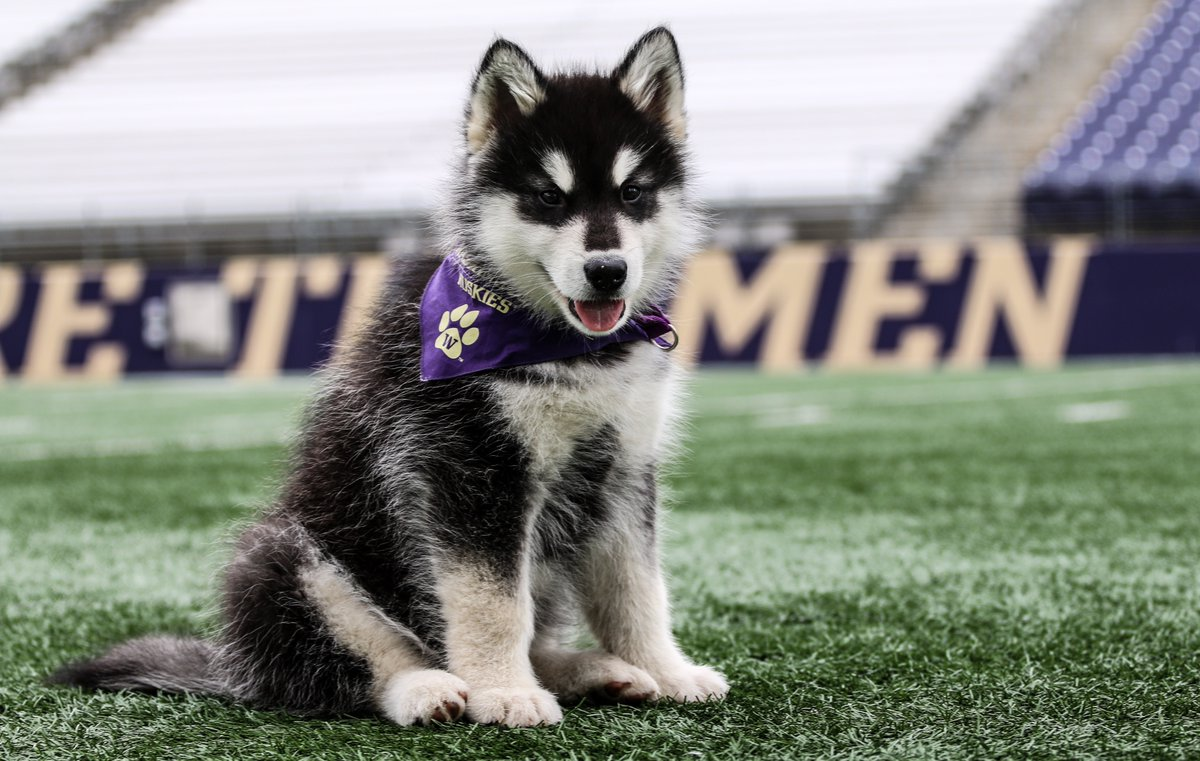
\includegraphics[width=0.5\linewidth]{dubs.jpg}
%     \caption{Here is a picture of Dubs \cite{webeck_2018}. Dubs did not swallow a marble.}
%     \label{fig:dubs}
% \end{figure}

% Summary and Conclusions
\newpage
\section{Summary and Conclusions}
Add your summary and conclusions here.

% References
\printbibliography

% Appendices
\begin{appendices}

% MATLAB Functions
% \section{MATLAB Functions}
% Add your important MATLAB functions here with a brief implementation explanation. This is how to make an \textbf{unordered} list:
% \begin{itemize}
%     \item \texttt{y = linspace(x1,x2,n)} returns a row vector of \texttt{n} evenly spaced points between \texttt{x1} and \texttt{x2}. 
%     \item \texttt{[X,Y] = meshgrid(x,y)} returns 2-D grid coordinates based on the coordinates contained in the vectors \texttt{x} and \texttt{y}. \text{X} is a matrix where each row is a copy of \texttt{x}, and \texttt{Y} is a matrix where each column is a copy of \texttt{y}. The grid represented by the coordinates \texttt{X} and \texttt{Y} has \texttt{length(y)} rows and \texttt{length(x)} columns.  
% \end{itemize}

% % MATLAB Codes
% \section{MATLAB Code}
% Add your MATLAB code here. This section will not be included in your page limit of six pages.

% \begin{listing}[h]
% \inputminted{matlab}{example.m}
% \caption{Example code from external file.}
% \label{listing:examplecode}
% \end{listing}

\end{appendices}

\end{document}
